\chapter{Građa uređaja}
\label{pog:structure}

Sustav se sastoji od dva uređaja koji zajedno rade u prikupljanju i obradi podataka. Središnji uređaj služi za snimanje, obradu i pohranu glasovnih podataka i obradu i pohranu biomedicinskih parametara. Za snimanje biomedicinskih parametara koristi se narukvica. Središnji uređaj i narukvica razmjenjuju podatke i naredbe putem Bluetooth protokola. Prikupljeni podaci se obrađuju pomoću neuralnih mreža kako bi se utvrdio intenzitet mucanja. Blok dijagram sustava prikazan je na slici \ref{slk:BD_MAIN}.
\begin{figure}[htb]
    \centering
    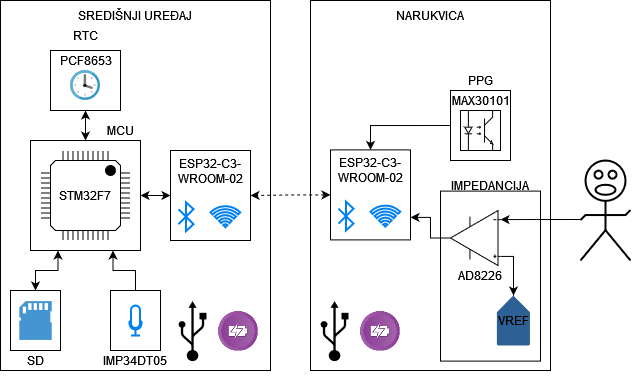
\includegraphics[width=\textwidth]{Figures/block_diagram.drawio.png}
    \caption{Blok dijagram sustava}
    \label{slk:BD_MAIN}
\end{figure}

Na središnjem uređaju nalazi se mikrokontroler (MCU) za obradu podataka, MEMS mikrofon za snimanje govora korisnika, SD kartica za lokalnu pohranu podataka i čip za praćenje vremena (RTC) za usklađivanje govornih podataka i biomedicinskih podataka. Podaci će se pohranjivati lokalno na uređaj kako bi logoped mogao kasnije preuzeti podatke te ih analizirati.

Narukvica mjeri brzinu otkucaja srca putem fotopletizmografskog senzora (PPG) i impedanciju kože s pomoću instrumentacijskog pojačala. Promjena impedancije kože je dobar pokazatelj stresa u korisnika \cite{edr}, a osobe s poremećajem tečnosti govora pokazuju značajno smanjenje brzine otkucaja srca u stresnim situacijama u odnosu na osobe bez takvih poremećaja \cite{ALM2004123}.

Oba uređaja sadržavaju sustav za bežičnu komunikaciju, baterijsko napajanje i mogućnost punjenja. Radi velike raširenosti koristit će se litij-ionska baterija i mogućnost punjenja putem USB C sučelja.

Zbog zahtjeva na nosivost uređaja, veličine tiskanih pločica (engl. \textit{Printed Circuit Board}, PCB), imaju ograničenje na fizičku veličinu, međutim, s obzirom na to da se radi o prototipu, uređaji će sadržavati testne točke i dovoljno velike komponente kako bi eventualna prerada pločice bila lakša. S obzirom na ta dva zahtjeva potrebno je napraviti pločicu koja će biti kompromis između ta dva zahtjeva.

Prvo će biti izrađen središnji sustav kako bi se ispitala mogućnost prikupljanja glasovnih podataka i sustav za napajanje na temelju čega će kasnije biti izrađena narukvica kako bi se upotpunile tražene funkcionalnosti sustava.